\documentclass[a4paper, 11pt, final]{article}

\usepackage{times}
\usepackage[IL2]{fontenc}
\usepackage[utf8]{inputenc}
\usepackage[czech]{babel}
\usepackage[left=2cm, text={17cm, 24cm}, top=3cm]{geometry}

\usepackage[unicode, hidelinks]{hyperref}
\urlstyle{same}

\usepackage{pdflscape}
\usepackage{graphicx}
\usepackage{xcolor}
\usepackage{mathtools}
\usepackage{siunitx}
\usepackage{multirow}

\providecommand{\uv}[1]{\quotedblbase #1 \textquotedblleft}

\usepackage{url}
\DeclareUrlCommand\url{\def\UrlLeft{<}\def\UrlRight{>} \urlstyle{tt}}

\usepackage{etoolbox}
\patchcmd{\thebibliography}{\section*{\refname}}{}{}{}

\usepackage{listings}
\definecolor{codegreen}{rgb}{0,0.6,0}
\definecolor{codegray}{rgb}{0.5,0.5,0.5}
\definecolor{codepurple}{rgb}{0.58,0,0.82}
\definecolor{backcolour}{rgb}{0.95,0.95,0.92}

\lstdefinestyle{mystyle}{
    backgroundcolor=\color{backcolour},   
    commentstyle=\color{codegreen},
    keywordstyle=\color{magenta},
    numberstyle=\tiny\color{codegray},
    stringstyle=\color{codepurple},
    basicstyle=\ttfamily\footnotesize,
    breakatwhitespace=false,         
    breaklines=true,                 
    captionpos=b,                    
    keepspaces=true,                 
    numbers=left,                    
    numbersep=5pt,                  
    showspaces=false,                
    showstringspaces=false,
    showtabs=false,                  
    tabsize=4
}

\lstset{style=mystyle}
\renewcommand{\lstlistingname}{Zdrojový kód}

\begin{document}

\begin{titlepage}
\begin{center}
    \Huge \textsc{Vysoké učení technické v~Brně}\\
    \huge \textsc{Fakulta informačních technologií}
    
    \vspace{\stretch{0.382}}
    
    \LARGE Signály a~systémy\\
    \Huge Protokol k~závěrečnému projektu
    
    \vspace{\stretch{0.618}}
\end{center}

\Large \noindent 31. prosince 2021 \hfill Michal Šmahel (xsmahe01)
\end{titlepage}

\section{Úvod}

Tento dokument slouží jako protokol k~závěrečnému projektu z~předmětu Signály a~systémy (ISS). Cílem projektu byla filtrace nežádoucích harmonicky vztažených kosinusovek ze zadaného zvukového signálu. Úkolem tedy bylo nalézt dané kosinusovky pomocí analýzy signálu a~navrhnout vhodný filtr (či více filtrů) pro jejich odfiltrování ze zadaného signálu.

Pro řešení projektu jsem využil programovací jazyk Python a~knihovny Numpy \cite{numpy-reference} a~Scipy (zejména modul signal) \cite{scipy-reference} pro matematické výpočty a~práci se signály, Matplotlib \cite{matplotlib-reference} pro tvorbu grafů, Soundfile \cite{soundfile-reference} pro práci s~WAV soubory a~Shutil \cite{shutil-reference} pro vysokoúrovňovou práci se soubory.

Pokud není uvedeno jinak, čerpám z~přednášek a~cvičení předmětu Signály a~systémy, studijní etapy k~projektu \cite{study-phase} a~její verze pro Python od Ing.~Kateřiny Žmolíkové \cite{zmolikova-demo}.

\section{Vypracování projektu}

V~této sekci bych rád popsal, jak jsem projekt řešil. Jednotlivé podsekce odpovídají úkolům ze zadání, číslování i~názvy podsekcí jsou identické.

\subsection{Základy}

Nejprve je třeba načíst zadaný signál. Ten je obsažen v~souboru typu WAV. Pro načtení signálu a~vzorkovací frekvence je vhodné použít knihovnu SoundFile \cite{soundfile-reference} (viz zdrojový kód \ref{code:load-file}). Po načtení totiž není třeba provádět normalizaci \cite{zmolikova-demo}.

\begin{lstlisting}[language=Python, caption=Načtení signálu z~WAV souboru, label={code:load-file}]
import numpy as np
import soundfile as sf

signal: np.ndarray
sample_rate: int
signal, sample_rate = sf.read(src_file)
\end{lstlisting}

Dále je třeba zjistit základní informace o~načteném signálu, jako je počet vzorků, délka v~sekundách a~minimální a~maximální hodnota. Tyto údaje se dají získat z~dat, které máme načtené ze souboru se signálem. Délka signálu v~sekundách se poté dopočítá pomocí vztahu $t = N / f_s$, kde $N$ je počet vzorků a~$f_s$ vzorkovací frekvence. Zjištěné hodnoty z~mého signálu jsou uvedeny v~tabulce \ref{tab:signal-info}.

\begin{table}[ht]
    \centering
    \begin{tabular}{|l|c|}
        \hline
        Počet vzorků & 41165 \\
        Délka signálu (s) & 2.57 \\
        Minimální hodnota & -0.2032 \\
        Maximální hodnota & 0.2319 \\
        \hline
    \end{tabular}
    \caption{Základní informace o~signálu (zaokrouhleno)}
    \label{tab:signal-info}
\end{table}

Nakonec zbývá si signál zobrazit v~grafu. Toho lze docílit poměrně jednoduše pomocí knihovny Matplotlib \cite{matplotlib-reference} (viz zdrojový kód \ref{code:plot-signal}). Kvůli tomu, že je obrázek dále vkládán do tohoto prokolu, je nutné oříznout bílou plochu okolo, to zajišťují parametry \texttt{bbox\_inches=”tight”} a~\texttt{pad\_inches=0} na řádku 11 \cite{zmolikova-demo}. Výsledný graf pro můj signál je na obrázku \ref{fig:signal-graph}). Z~obrázku je patrné, že je signál určitým způsobem zarušen, podle obdélníku obsaženého v~grafu. Ten se pohybuje vertikální ose mezi hodnotami cca $0.02$ až $0.05$. V~grafu vyfiltrovaného signálu (viz obrázek \ref{fig:filtered-signal-graph}) již tento obdélník obsažen není.

\begin{lstlisting}[language=Python, caption=Vykreslení grafu signálu do PDF souboru, label={code:plot-signal}]
import matplotlib.pyplot as plt

samples = signal.size
time_axis = np.arange(samples) / sample_rate

plt.figure()
plt.plot(time_axis, signal)

plt.gca().set_xlabel("Cas $[s]$")

plt.tight_layout()
plt.savefig("input-signal.pdf", bbox_inches="tight", pad_inches=0)
plt.close()
\end{lstlisting}

\begin{figure}[ht]
    \centering
    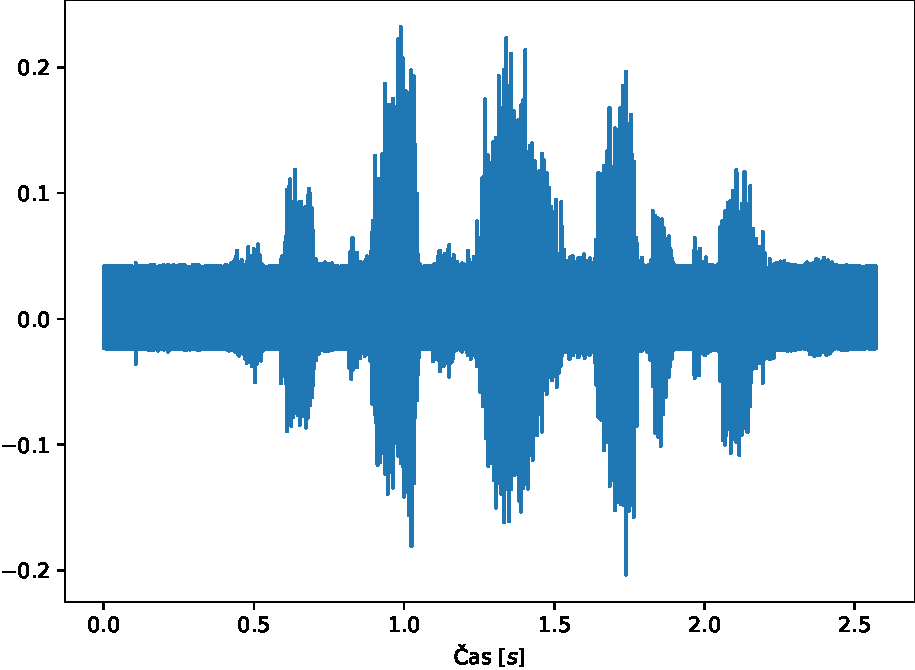
\includegraphics{img/01-input-signal.pdf}
    \caption{Graf vstupního signálu}
    \label{fig:signal-graph}
\end{figure}

\subsection{Předzpracování a~rámce}

Pro další práci se signálem je nejprve nutné provést několik přípravných kroků. Nejprve se signál ustřední, čehož docílíme pomocí odečtení střední hodnoty. Nejprve spočítáme střední hodnotu a následně ji odečteme od~signálu. K~tomu využijeme knihovnu Numpy \cite{numpy-reference} (viz zdrojový kód \ref{code:centralization}).

\begin{lstlisting}[language=Python, caption=Ustřednění signálu, label={code:centralization}]
mid_val = np.mean(signal)
signal_centered = np.subtract(signal, mid_val)
\end{lstlisting}

Dále je třeba signál znormovat, tedy dostat jeho hodnoty do intervalu $\left<-1, 1\right>$. Toho docílíme opět pomocí knihovny Numpy \cite{numpy-reference} (viz \ref{code:normalization}). Výpočet je prostý -- na signál aplikujeme absolutní hodnotu pro získání maximální hodnoty nehledě na znaménko a poté maximální hodnotou původní signál vydělíme.

\begin{lstlisting}[language=Python, caption=Normalizace signálu, label={code:normalization}]
signal_abs = np.abs(signal_centered)
abs_max_val = np.max(signal_abs)
signal_norm = np.divide(signal_centered, abs_max_val)
\end{lstlisting}

Dále si signál rozdělíme na překrývající se rámce o~délce 1024 vzorků s~překrytím přes 512 vzorků (viz zdrojový kód \ref{code:creating-frames}). Jelikož je budeme potřebovat v~následující podsekci, kde budeme počítat diskrétní Fourierovu transformaci (DFT) pomocí matic a vektorů, uložíme si je sloupcově (viz řádek 6) \cite{numpy-reference}. Celý proces je poměrně zřejmý, takže nepotřebuje větší komentář. Za zmínku stojí asi jen to, že se v~případě posledního rámce, který může být kratší, doplní zbylé vzorky hodnotou $0$ (viz řádek 4) \cite{numpy-reference}.

\begin{lstlisting}[language=Python, caption=Rozdělení na překrývající se rámce, label={code:creating-frames}]
frames = []
for frame_num in range(round(samples / frame_overlap)):
    frame = np.array(signal_norm[frame_num * frame_overlap:frame_num * frame_overlap + frame_size])
    frame = np.pad(frame, (0, frame_size - frame.size), 'constant')
    frames.append(frame)
frames_cols = np.column_stack(frames)
\end{lstlisting}

Z~vytvořených rámců je možné vybrat nějaký \uv{znělý}, který má relativně zachovanou periodicitu. Podle tohoto rámce jde následně např. odhadovat rušivé frekvence pomocí DFT. Ze svého signálu jsem vybral rámec č. 42, jehož graf je na obrázku \ref{fig:nice-frame}.

\begin{figure}[ht]
    \centering
    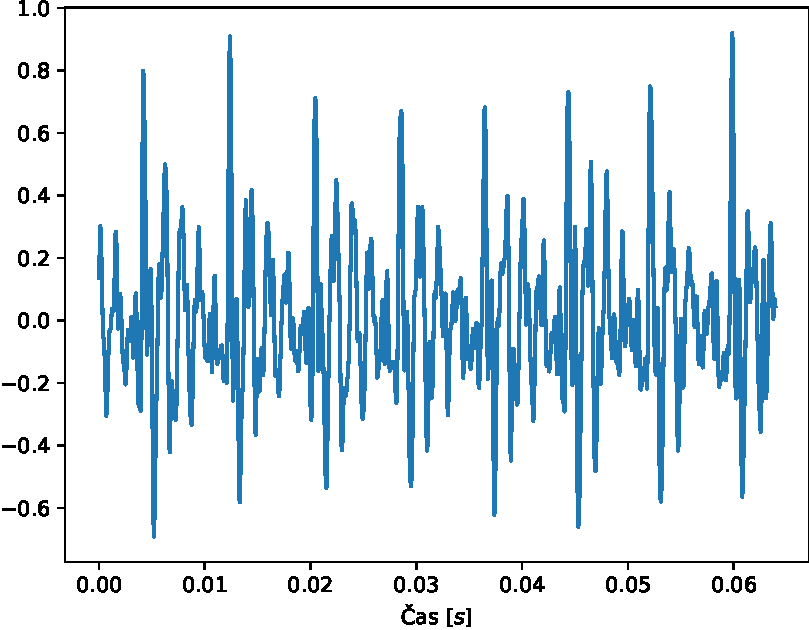
\includegraphics{img/02-nice-frame.pdf}
    \caption{Graf \uv{znělého} rámce}
    \label{fig:nice-frame}
\end{figure}

\subsection{DFT}

Jak již bylo zmíněno v~předchozí podsekci, pomocí DFT (diskrétní Fourierovy transformace) je možné signál analyzovat. Konkrétně se jedná o~analýzu ve frekvencích, což se hodí např. pro vyhledání rušivých frekvencí, které trápí náš signál. V~Pythonu se pro výpočet DFT běžně používá funkce \texttt{np.fft.fft()}, tedy rychlá Fourierova transformace, což je rychlejší algoritmus pro výpočet DFT \cite{zmolikova-demo}.

Úkolem v~tomto projektu bylo mimo jiné implementovat vlastní funkci pro výpočet DFT pomocí maticových výpočtů a porovnat ji se zmíněnou funkcí \texttt{np.fft.fft()} z~knihovny Numpy \cite{numpy-reference}. Při implementaci vlastní funkce pro maticový výpočet DFT jsem využil poznatky a~vzorce z~prezentace dr.~Mautnera \cite{dft-matrix} (viz zdrojový kód \ref{code:dft}). Obrázek \ref{fig:dft-graph-comparison} zachycuje výsledky obou funkcí a tabulka \ref{tab:dft-time-comparison} zobrazuje porovnání rychlostí obou postupů.

\begin{lstlisting}[language=Python, caption=Vlastní funkce pro výpočet DFT, label={code:dft}]
def dft(signal: np.array) -> np.array:
    N = signal.size
    w = np.exp(-2j * np.pi / N)

    base_matrix = []
    for i in range(0, N):
        row = []
        for j in range(0, N):
            row.append(np.power(w, i * j))
        base_matrix.append(row)

    base_matrix = np.array(base_matrix)

    return np.dot(base_matrix, signal)
\end{lstlisting}

\begin{figure}[ht]
    \centering
    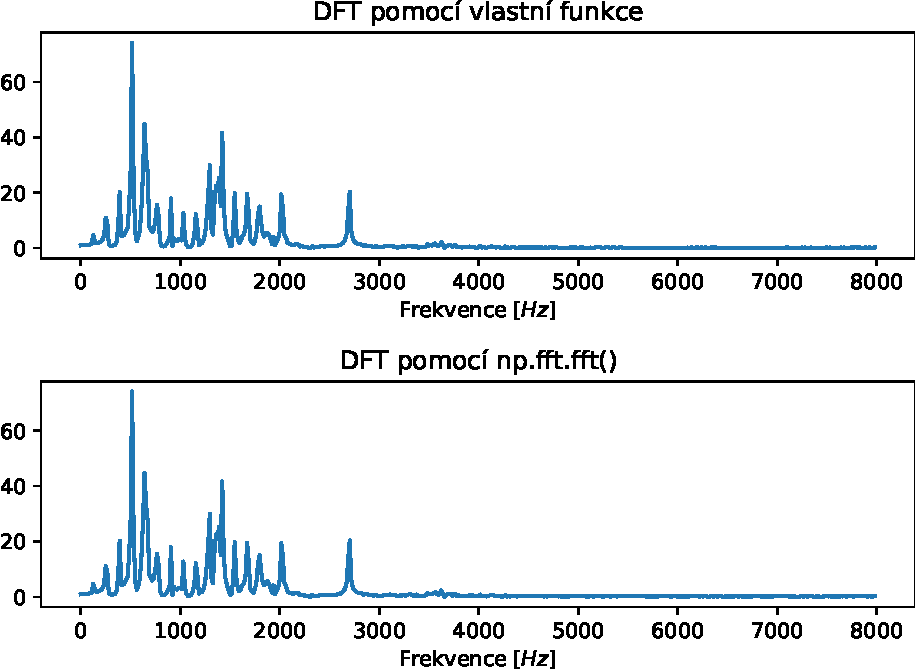
\includegraphics{img/03-dft-module.pdf}
    \caption{Porovnání výsledků \texttt{np.fft.fft()} s~vlastní funkcí\protect\footnotemark}
    \label{fig:dft-graph-comparison}
\end{figure}
\footnotetext{Zobrazeny jsou pouze moduly komplexních čísel.}

\begin{table}[ht]
    \centering
    \begin{tabular}{|l|c|}
        \hline
        \texttt{np.fft.fft()} & $\SI{56.97}{\micro\second}$ \\
        Vlastní funkce & $\SI{3.86}{\second}$ \\
        \hline
    \end{tabular}
    \caption{Časy výpočtu DFT (zaokrouhleno)}
    \label{tab:dft-time-comparison}
\end{table}

\subsection{Spektrogram}

Klíčovým krokem při práci na tomto projektu je vygenerování logaritmického výkonového spektrogramu. Z~něho je velmi dobře patrné, jak signál vypadá (z~frekvenčního hlediska), a kde (resp. na jakých frekvencích) se přibližně pohybují rušivé frekvence.

Spektrogram je generován pomocí knihovny Scipy \cite{scipy-reference} a Numpy \cite{numpy-reference} a zobrazený pomocí knihovny Matplotlib~\cite{matplotlib-reference} s~využitím postupu z~materiálů Ing. Žmolíkové \cite{zmolikova-demo} (viz zdrojový kód \ref{code:spectrogram}).

\begin{lstlisting}[language=Python, caption=Zobrazení spektrogramu zadaného signálu, label={code:spectrogram}]
freq_axis, time_axis, sgr = spectrogram(signal, sample_rate, nperseg=frame_size, noverlap=frame_overlap)
sgr_log = 10 * np.log10(sgr + 1e-20)

plt.figure(figsize=(9, 5))

plt.pcolormesh(time_axis, freq_axis, sgr_log)
plt.gca().set_xlabel("Cas $[s]$")
plt.gca().set_ylabel("Frekvence $[Hz]$")
cbar = plt.colorbar()
cbar.set_label("Spektralni hustota vykonu $[dB]$", rotation=270, labelpad=15)

plt.tight_layout()
plt.savefig("spectrogram.pdf", bbox_inches="tight", pad_inches=0)
\end{lstlisting}

\begin{figure}[ht]
    \centering
    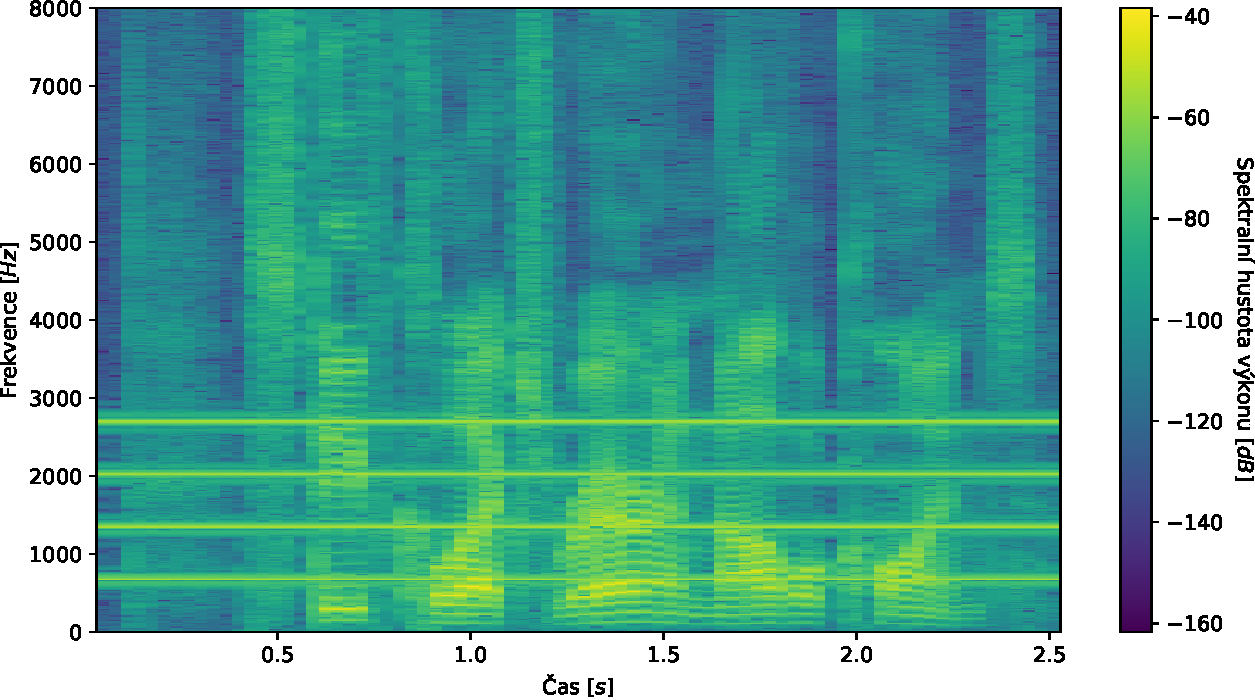
\includegraphics[width=\textwidth]{img/04-spectrogram.pdf}
    \caption{Logaritmický výkonový spektrogram zadaného signálu}
    \label{fig:signal-spectrogram}
\end{figure}

Výsledný spektrogram je možné vidět na obrázku \ref{fig:signal-spectrogram}. Při pohledu na něho je zřejmé, že signál obsahuje 4 kosinusovky (žluté horizontální proužky) na frekvencích v~rozmezí $\left(0, 3000\right) \si{\hertz}$. Tato znalost se bude hodit v~následujícím kroku.

\subsection{Určení rušivých frekvencí}

Nyní nastal čas určit rušivé frekvence, které budeme následně filtrovat. Je mnoho možností, jak tyto frekvence zjistit. Při svém řešení jsem vyzkoušel dvě velmi triviální metody, z~nichž druhá měla poměrně rozumné výsledky, a tak jsem se rozhodl, že již další metody zkoušet nebudu. Pokud by druhá příliš neuspěla, dále jsem měl v~plánu využít vyčítání frekvencí z~DFT průměrného rámce, což jsem později objevil v~dostupných materiálech \cite{zmolikova-demo}.

Nejprve jsem frekvence získávat poloautomatickou metodou založenou na analýze \uv{znělého} rámce. Pro~tento rámec (jehož graf je na obrázku \ref{fig:nice-frame}) jsem spočítal DFT a následně pomocí funkce \texttt{find\_peaks()} z~knihovny Scipy nalezl souřadnice výkyvů \cite{scipy-reference}. Ty jsem si vypsal a v~grafu DFT (viz obrázek \ref{fig:nice-frame-dft}) si zvýraznil jejich umístění, abych k~bodům v~grafu mohl přiřadit vypsané hodnoty. Aplikací této metody jsem získal frekvence zobrazené v~tabulce \ref{tab:freq-list-1st-method}. Výsledky nejsou příliš přesné, takže jsem přistoupil k~druhé metodě.

\begin{figure}[ht]
    \centering
    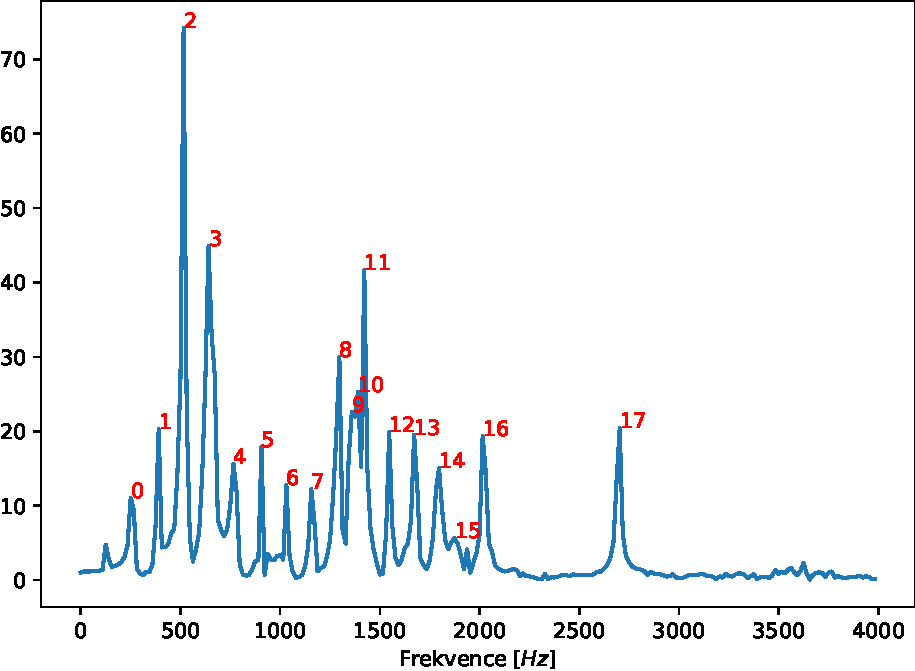
\includegraphics{img/05-nice-frame-dft.pdf}
    \caption{DFT \uv{znělého} rámce s~vyznačenými zajímavými výkyvy}
    \label{fig:nice-frame-dft}
\end{figure}

\begin{table}[ht]
    \centering
    \begin{tabular}{|c|c|}
        \hline
        \textbf{Frekvence $[\si{\hertz}]$} & \textbf{Násobek (cca)} \\
        \hline
        $640.625$ & $1\times$ \\
        $1359.375$ & $2\times$ \\
        $2015.625$ & $3\times$ \\
        $2703.125$ & $4\times$ \\
        \hline
    \end{tabular}
    \caption{Rušivé frekvence získané první metodou}
    \label{tab:freq-list-1st-method}
\end{table}

Druhá metoda spočívá v~manuálním odečtení hodnot ze spektrogramu s~dostatečnou přesností. Z~první metody jsem věděl, kde zhruba se rušivé frekvence objevují, díky čemuž jsem mohl poměrně přesně zaměřit na~odpovídající části spektrogramu načteného signálu. To je možné zařídit pomocí omezení zobrazené části grafu a změny měřítka osy (viz zdrojový kód \ref{code:detailed-graph-values}) \cite{matplotlib-reference}.

\begin{lstlisting}[language=Python, caption=Zobrazení detailního pohledu na spektrogram, label={code:detailed-graph-values}]
plt.pcolormesh(time_axis, freq, sgr_log)
plt.set_xlabel('Cas $[s]$')
plt.set_ylabel('Frekvence $[Hz]$')
plt.set_ylim(bottom=600, top=700)
plt.yaxis.set_major_locator(ticker.MultipleLocator(25))
\end{lstlisting}

Takto jsem si nechal zobrazit 4 úseky, v~nichž jsem očekával rušivé frekvence. Vznikl tak obrázek \ref{fig:detailed-spectrogram}, z~něhož jen stačí odečíst hodnoty rušivých frekvencí. Ty jsou vypsány v~tabulce \ref{tab:freq-list-2nd-method}. Stále jsou frekvence určovány pouze s~přesností $\SI{25}{\hertz}$, ale po aplikaci čistících filtrů v~posledním kroku se zdá, že je to dostatečné.

\begin{figure}[ht]
    \centering
    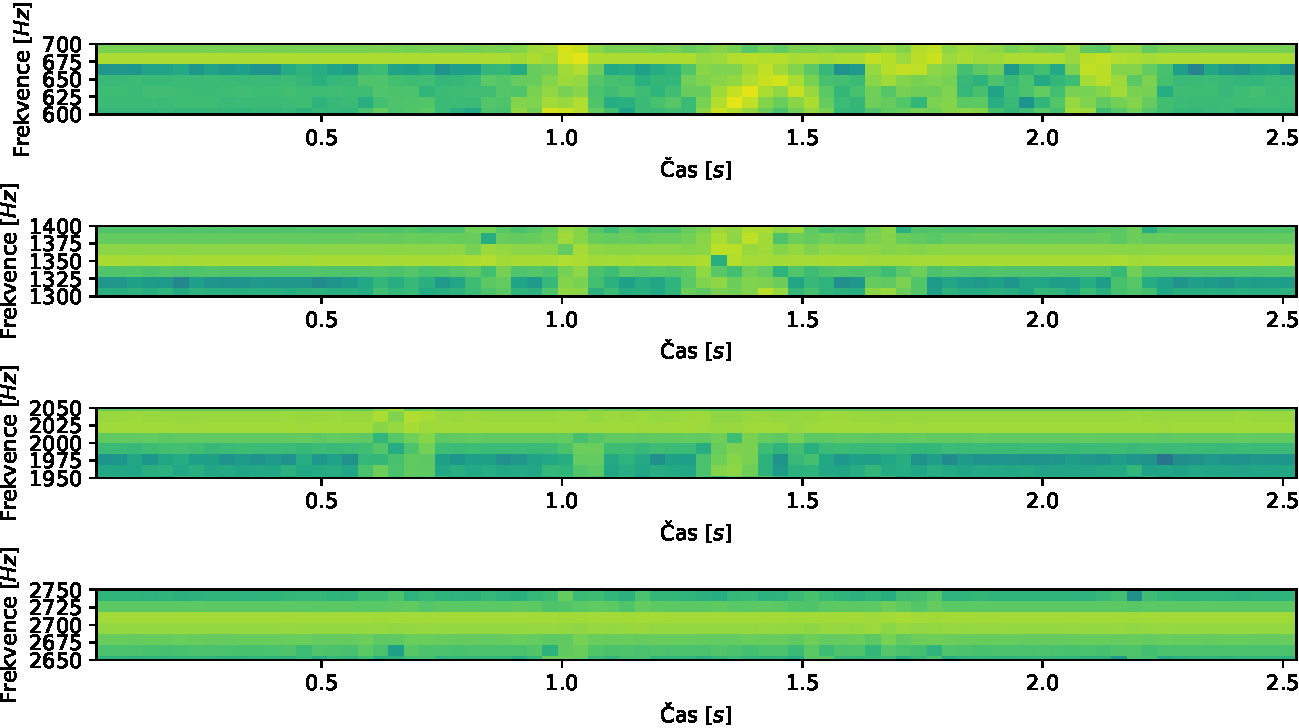
\includegraphics[width=\textwidth]{img/05-detailed-spectrogram.pdf}
    \caption{Detailně zaměřené části spektrogramu zadaného signálu}
    \label{fig:detailed-spectrogram}
\end{figure}

\begin{table}[ht]
    \centering
    \begin{tabular}{|c|c|}
        \hline
        \textbf{Frekvence $[\si{Hz}]$} & \textbf{Násobek} \\
        \hline
        $675$ & $1\times$ \\
        $1350$ & $2\times$ \\
        $2025$ & $3\times$ \\
        $2700$ & $4\times$ \\
        \hline
    \end{tabular}
    \caption{Rušivé frekvence získané ze spektrogramu}
    \label{tab:freq-list-2nd-method}
\end{table}

\subsection{Generování signálu}

Ještě než proběhne návrh filtrů a samotná filtrace, je možné vygenerovat si signál obsahující pouze ony rušivé kosinusovky na nalezených frekvencích (viz tabulka \ref{tab:freq-list-2nd-method}). To je možné např. pomocí funkce \texttt{chirp()} z~knihovny SciPy \cite{scipy-reference}. Ta umí generovat různé signály s~proměnlivými frekvencemi. Pro naše účely však stačí využít konfiguraci uvedenou ve zdrojovém kódu \ref{code:cos-gen} na řádku 3. Výsledný signál obsahující všechny kosinusovky je poté vytvářen součtem dosavadního signálu s~nově vygenerovanou kosinusovkou (viz řádek 8). První kosinusovka je signálu pouze přiřazena.

\begin{lstlisting}[language=Python, caption=Generování kosinusovek, label={code:cos-gen}]
cos_signal = []
for cos_freq in cos_frequencies:
    gen_signal = chirp(time_axis, f0=cos_freq, f1=cos_freq, t1=length, method='linear')

    if len(cos_signal) == 0:
        cos_signal = gen_signal
    else:
        cos_signal = np.add(cos_signal, gen_signal)
cos_signal = np.array(cos_signal)
\end{lstlisting}

Jak vypadají jednotlivé kosinusovky zachycuje obrázek \ref{fig:cos-signals-divided}. Jelikož používáme velké množství vzorků, není bohužel kosinusový průběh příliš viditelný. Lepší je prohlédnout si spektrogram na obrázku \ref{fig:cos-signals-spectrogram}, kde je pěkně vidět známé \uv{proužky} ze spektrogramu zadaného signálu (viz obrázek \ref{fig:signal-spectrogram}), které jsou tentokrát zcela osamocené.

\begin{figure}[ht]
    \centering
    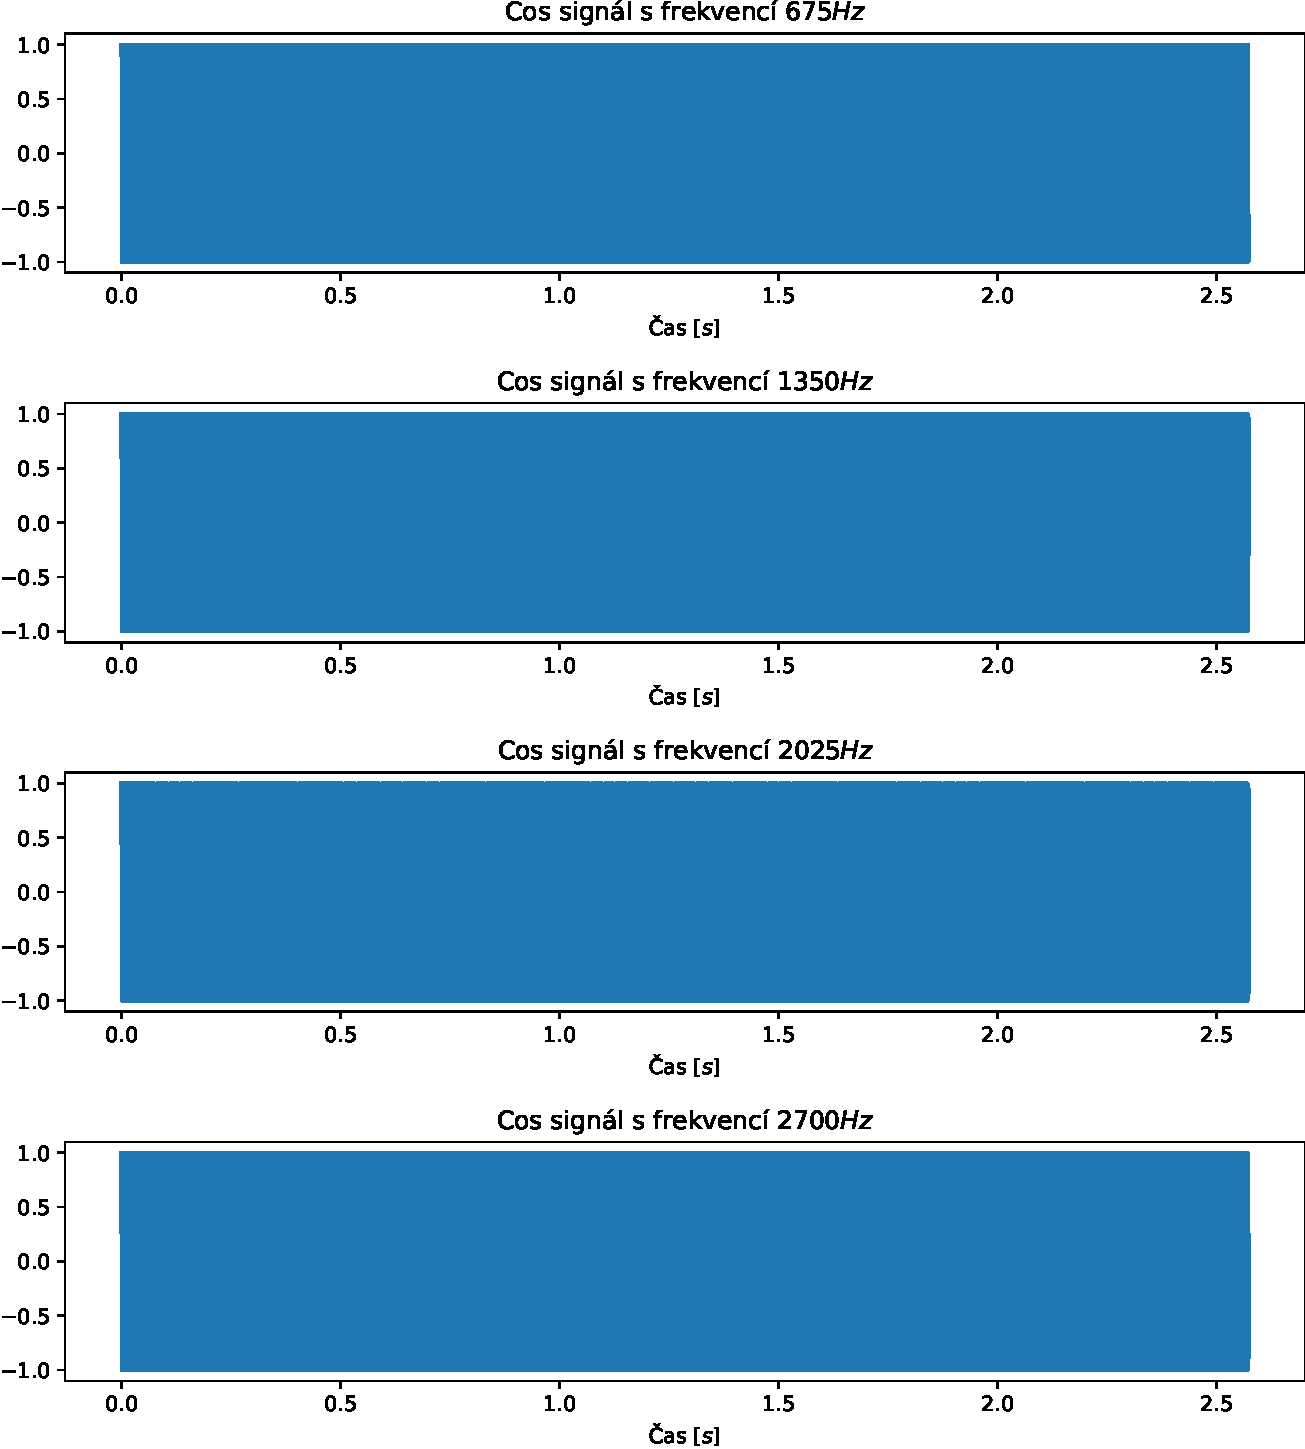
\includegraphics[scale=0.5]{img/06-cos-signals-divided.pdf}
    \caption{Jednotlivé rušivé kosinusovky}
    \label{fig:cos-signals-divided}
\end{figure}

\begin{figure}[ht]
    \centering
    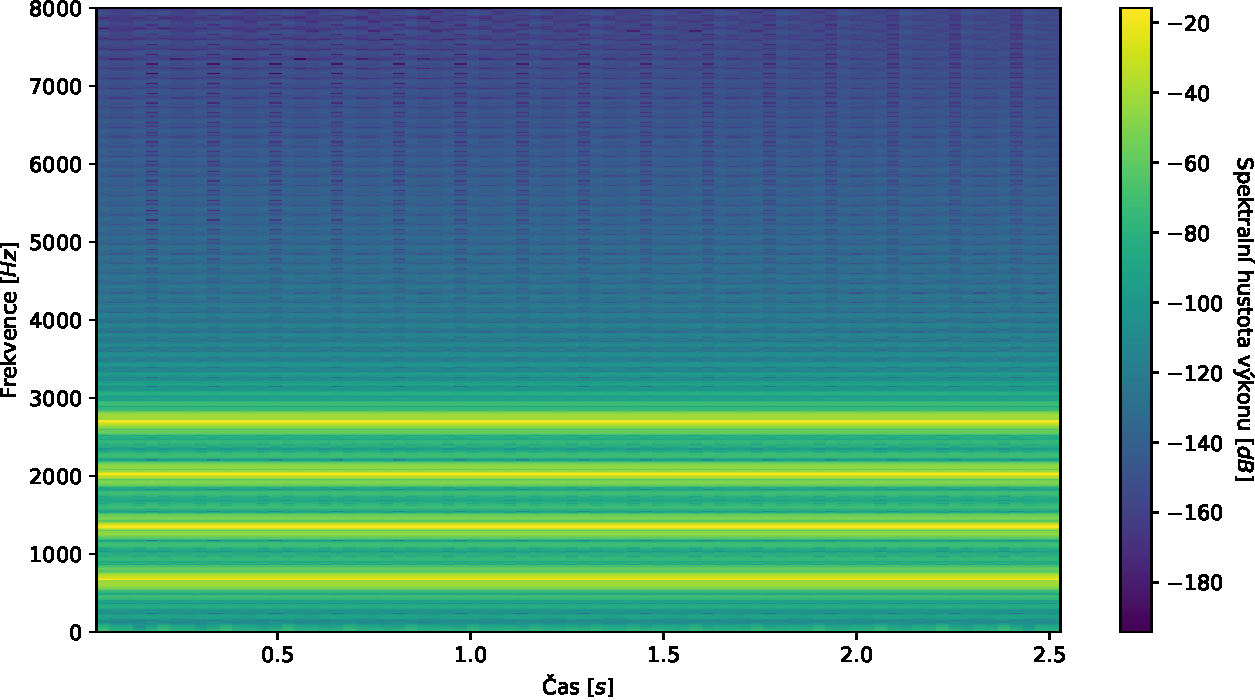
\includegraphics[width=\textwidth]{img/06-cos-signals-spectrum.pdf}
    \caption{Spektrogram rušivých kosinusovek}
    \label{fig:cos-signals-spectrogram}
\end{figure}

Vygenerovaný signál je také možné uložit do WAV souboru. Toho se docílí, podobně jako v~případě načtení zadaného signálu, pomocí knihovny SoundFile \cite{soundfile-reference}. Operace je zachycena ve zdrojovém kódu \ref{code:save-signal}.

\begin{lstlisting}[language=Python, caption=Uložení signálu do WAV souboru, label={code:save-signal}]
sf.write("4cos.wav", cos_signal, sample_rate)
\end{lstlisting}

\subsection{Čistící filtr}

Nyní konečně nadešel čas na návrh filtrů. Pro tento krok jsem zvolil tvorbu 4 filtrů typu pásmová zádrž pomocí funkcí \texttt{buttord()} a \texttt{butter()} z~knihovny SciPy \cite{scipy-reference}. Při nastavování parametrů funkce \texttt{buttord()} jsem vycházel z~informací uvedených v~zadání. Vznikl tak zdrojový kód \ref{code:filter-coefficients}.

\begin{lstlisting}[language=Python, caption=Získání koeficientů filtrů, label={code:filter-coefficients}]
nyquist_freq = sample_rate / 2

filters = []
for cos_freq in cos_frequencies:
    lowest_ord, wn = buttord(
        wp=[(cos_freq - 50) / nyquist_freq, (cos_freq + 50) / nyquist_freq],
        ws=[(cos_freq - 15) / nyquist_freq, (cos_freq + 15) / nyquist_freq],
        gpass=3, gstop=40
    )

    b, a = butter(lowest_ord, wn, 'bandstop', output='ba')
    result_filter = (b, a)
    filters.append(result_filter)
filters = np.array(filters)
\end{lstlisting}

Filtry vygenerované pro zjištěné rušivé frekvence (viz tabulka \ref{tab:freq-list-2nd-method}) poté mají koeficienty zachycené v~tabulce \ref{tab:filter-coefficients}. Jejich impulsní odezvy jsou zobrazeny na obrázku \ref{fig:filter-impulse-responses}. Postup výpočtu a zobrazení impulsní odezvy je zachycen ve zdrojovém kódu \ref{code:filter-impulse-response}, byl víceméně převzat z~materiálů \cite{zmolikova-demo}.

\begin{lstlisting}[language=Python, caption=Výpočet a zobrazení impulsní odezvy filtrů, label={code:filter-impulse-response}]
for (b, a) in filters:
    unit_pulse = [1, *np.zeros(imp_res_samples - 1)]
    imp_res = lfilter(b, a, unit_pulse)

    plt.stem(np.arange(imp_res_samples), imp_res, basefmt=' ', use_line_collection=True)

    plt.set_xlabel('$n$')
    plt.set_title(f"Filtr pro frekvenci ${cos_frequencies[i]}\\ Hz$")
    plt.grid(alpha=0.5, linestyle='--')
\end{lstlisting}

\begin{figure}[!hp]
    \centering
    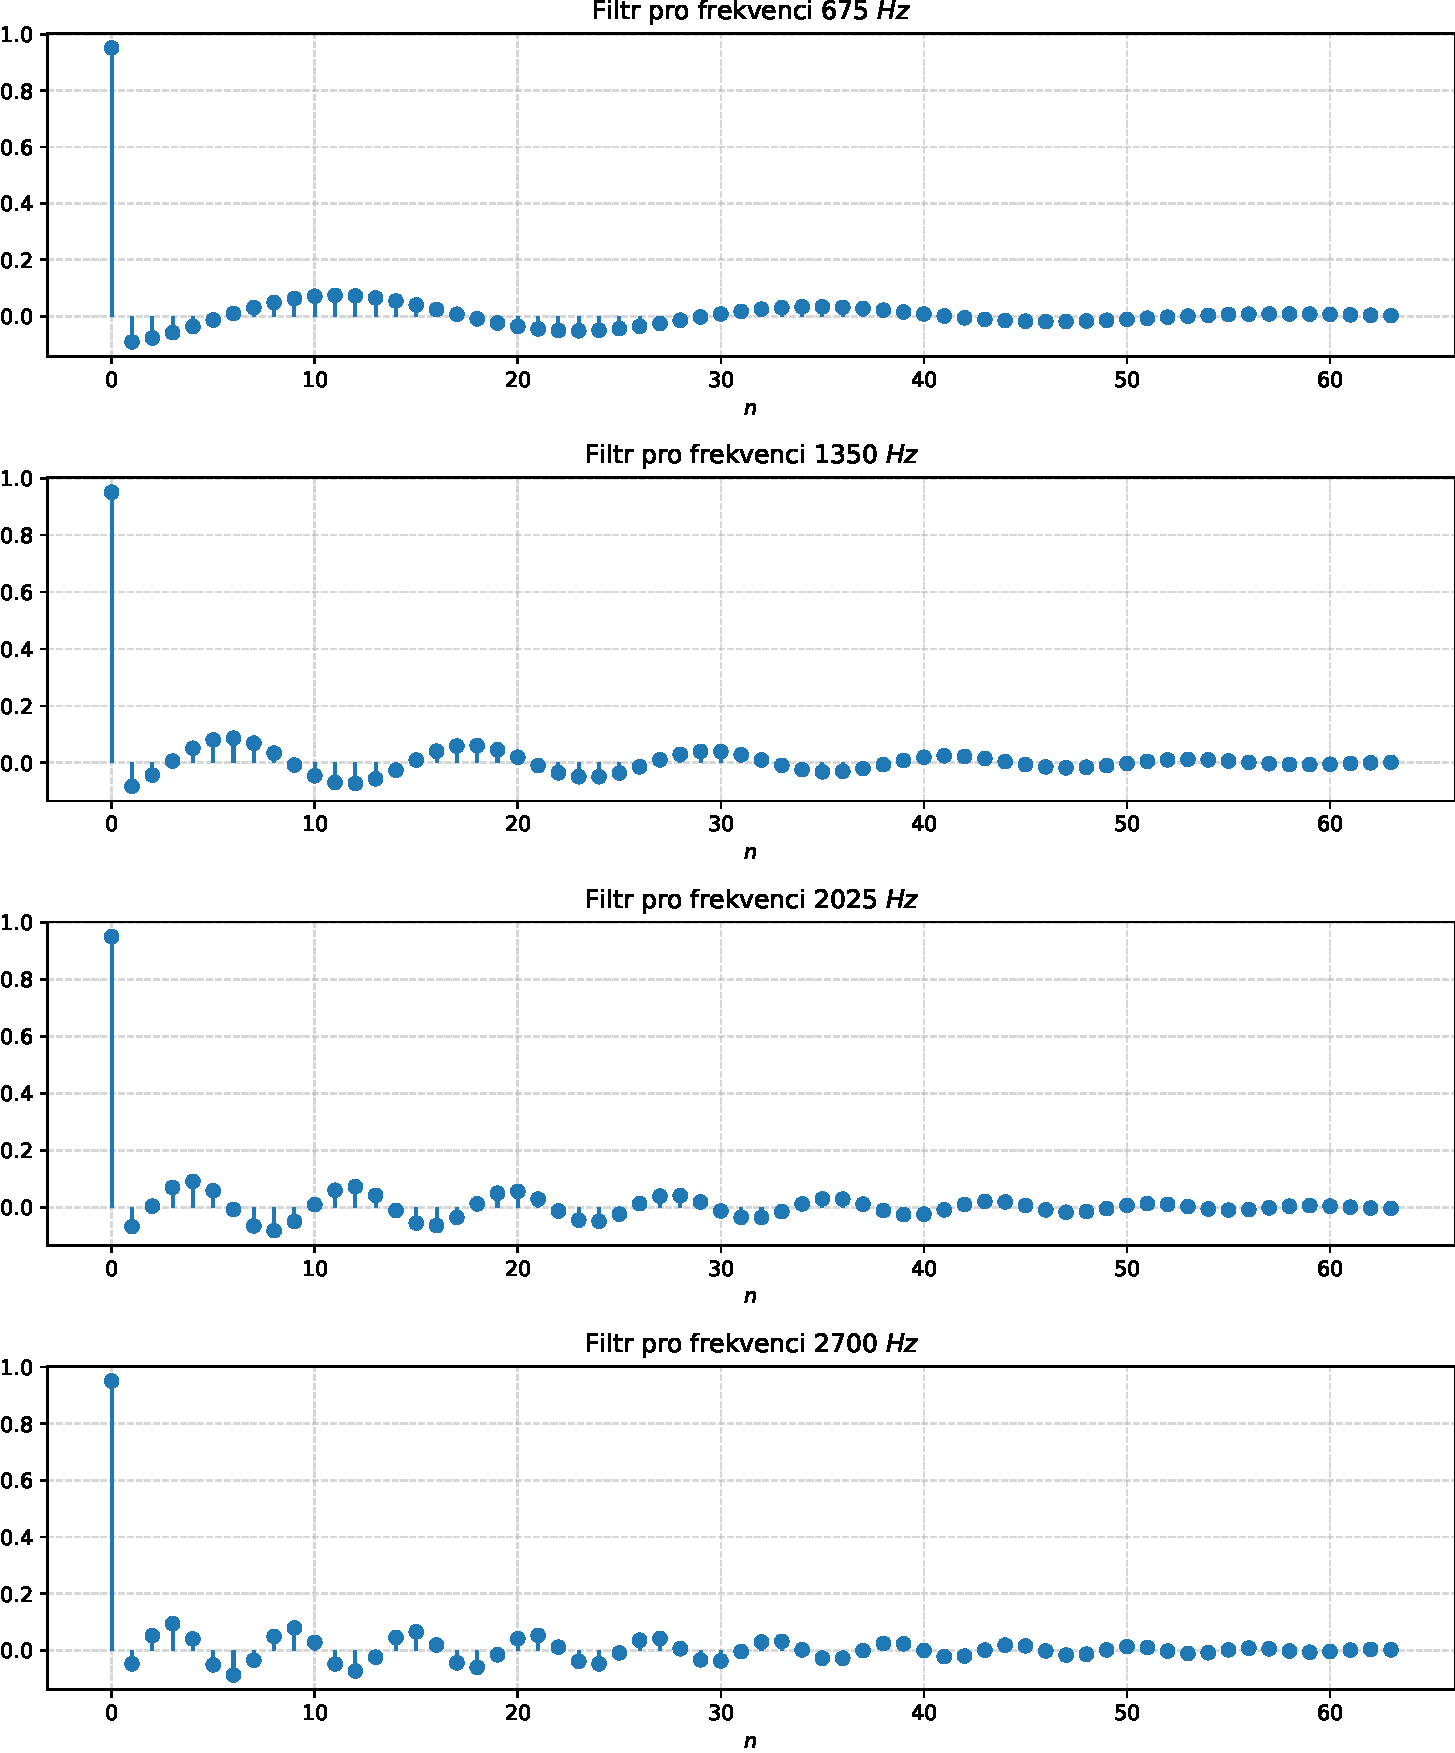
\includegraphics[width=\textwidth]{img/07-impulse-responses.pdf}
    \caption{Impulsní odezvy navržených filtrů}
    \label{fig:filter-impulse-responses}
\end{figure}

\begin{table}[!ht]
    \centering
    \begin{tabular}{|c|cl|}
        \hline
        \textbf{Filtr} & \multicolumn{2}{c|}{\textbf{Koeficienty}} \\
        \hline
        \multirow{2}{*}{$\SI{675}{\hertz}$} & \textbf{b} & $0.9515$, $-7.3464$, $25.0760$, $-49.4092$, $61.4563$, $-49.4092$, $25.0760$, $-7.3464$, $0.9515$ \\
            & \textbf{a} & $1.0000$, $-7.6248$, $25.7035$, $-50.0185$, $61.4452$, $-48.7909$, $24.4573$, $-7.0771$, $0.9054$ \\
        \hline
        \multirow{2}{*}{$\SI{1350}{\hertz}$} & \textbf{b} & $0.9507$, $-6.5620$, $20.7872$, $-39.2238$, $48.1011$, $-39.2238$, $20.7872$, $-6.5620$, $0.9507$ \\
            & \textbf{a} & $1.0000$, $-6.8149$, $21.3158$, $-39.7148$, $48.0914$, $-38.7243$, $20.2658$, $-6.3176$, $0.9039$ \\
        \hline
        \multirow{2}{*}{$\SI{2025}{\hertz}$} & \textbf{b} & $0.9504$, $-5.3236$, $14.9835$, $-26.4092$, $31.7204$, $-26.4092$, $14.9835$, $-5.3236$, $0.9504$ \\
            & \textbf{a} & $1.0000$, $-5.5300$, $15.3668$, $-26.7413$, $31.7131$, $-26.0702$, $14.6051$, $-5.1240$, $0.9033$ \\
        \hline
        \multirow{2}{*}{$\SI{2700}{\hertz}$} & \textbf{b} & $0.9503$, $-3.7146$, $9.2463$, $-14.6915$, $17.4588$, $-14.6915$, $9.2463$, $-3.7146$, $0.9502$ \\
            & \textbf{a} & $1.0000$, $-3.8592$, $9.4833$, $-14.8765$, $17.4540$, $-14.5018$, $9.0116$, $-3.5749$, $0.9030$ \\
        \hline
    \end{tabular}
    \caption{Koeficienty navržených filtrů (zaokrouhleno)\protect\footnotemark}
    \label{tab:filter-coefficients}
\end{table}
\footnotetext{Filtry jsou nazvány podle frekvencí, které mají ze signálu vyfiltrovat.}

\subsection{Nulové body a~póly}

Pro navržené filtry je dále vhodné vypočítat nuly a póly a zobrazit si je na jednotkové kružnici v~komplexní rovině. Díky tomu je možné jednoduše ověřit, zda jsou navržené filtry stabilní. Nuly a póly je možné vypočítat pomocí funkce \texttt{tf2zpk()} z~knihovny SciPy \cite{scipy-reference}. Jejich zobrazení je poté možné pomocí postupu z~materiálů \cite{zmolikova-demo} s~využitím knihovny Matplotlib \cite{matplotlib-reference}. Grafy je možné vidět na obrázku \ref{fig:zeros-poles}.

\begin{figure}[ht]
    \centering
    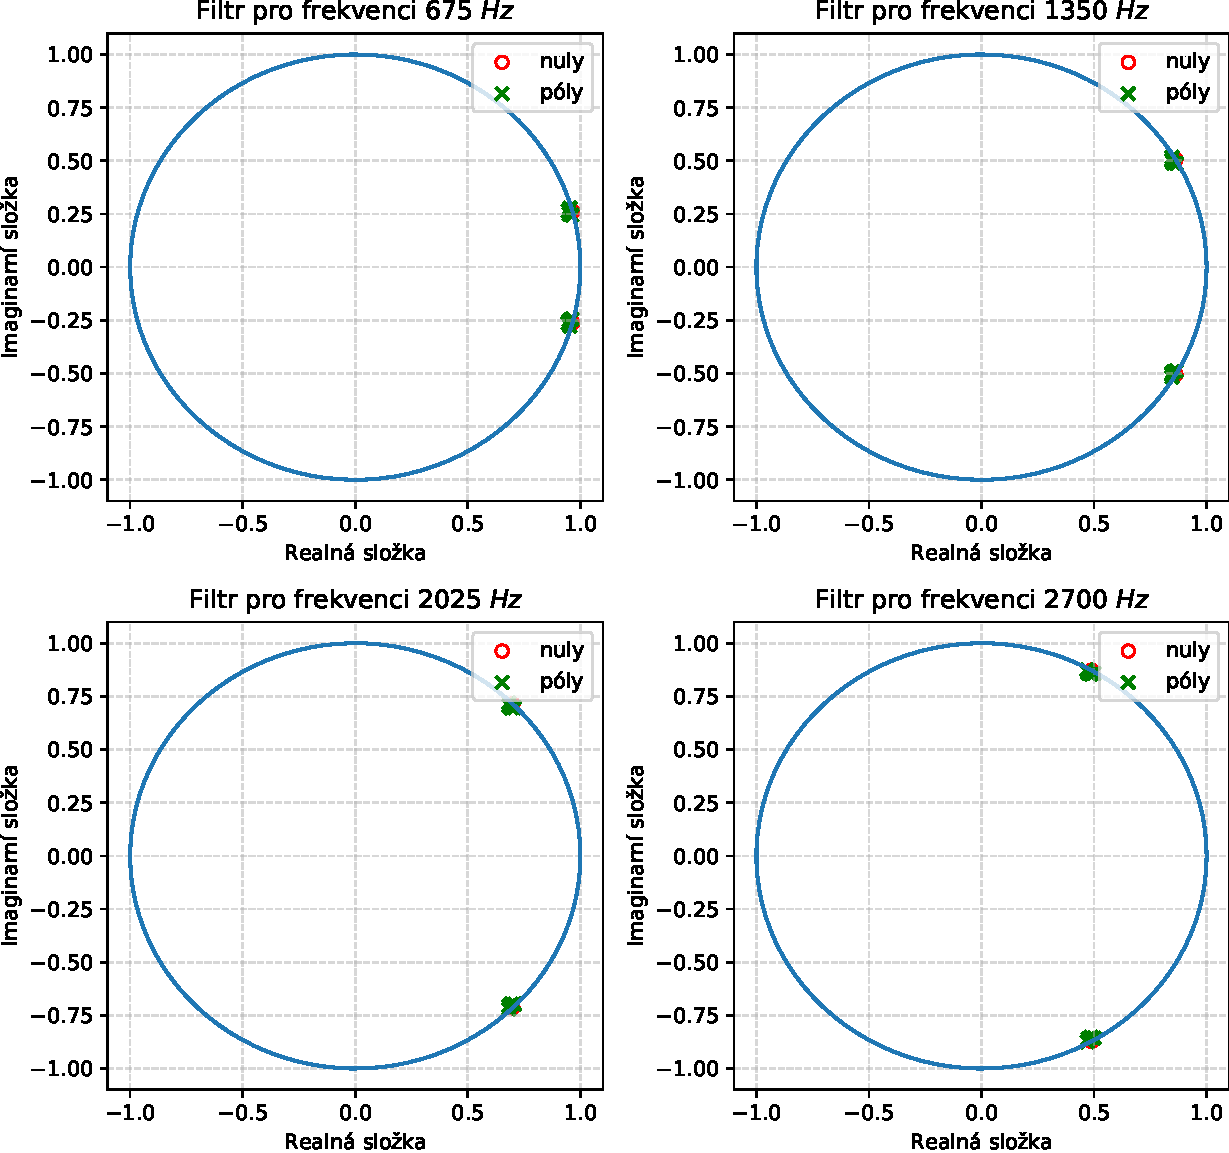
\includegraphics[scale=0.6]{img/08-zeros-poles.pdf}
    \caption{Nulové body a póly navržených filtrů}
    \label{fig:zeros-poles}
\end{figure}

Jak je možné vidět na obrázku \ref{fig:zeros-poles}, komplexní roviny jsou po dvou na řádku. To je z~toho důvodu, aby se uspořilo místo a obrázek se nemusel rozkládat na několik částí. Z~tohoto důvodu bylo třeba rozšířit kód pro~vykreslování grafů uvedený ve zdrojovém kódu \ref{code:plot-signal} \cite{matplotlib-reference}. Konkrétní řešení je uvedeno ve zdrojovém kódu \ref{code:filter-zeros-poles}.

\begin{lstlisting}[language=Python, caption=Výpočet a zobrazení nul a pólů navržených filtrů, label={code:filter-zeros-poles}]
    fig, axes = plt.subplots(2, 2, figsize=(8.5, 8))

    i = 0
    j = 0
    for (b, a) in filters:
        zeros, poles, _ = tf2zpk(b, a)

        ang = np.linspace(0, 2 * np.pi, 100)
        axes[i][j].plot(np.cos(ang), np.sin(ang))

        axes[i][j].scatter(np.real(zeros), np.imag(zeros), marker="o", facecolors="none", edgecolors="r", label="nuly")
        axes[i][j].scatter(np.real(poles), np.imag(poles), marker="x", color="g", label="poly")

        axes[i][j].set_xlabel("Realna slozka")
        axes[i][j].set_ylabel("Imaginarni slozka")
        axes[i][j].set_title(f"Filtr pro frekvenci ${cos_frequencies[2 * i + j]}\\ Hz$")
        axes[i][j].grid(alpha=0.5, linestyle="--")
        axes[i][j].legend(loc="upper right")

        j += 1
        if j >= 2:
            i += 1
            j = 0
\end{lstlisting}

\subsection{Frekvenční charakteristika}

Pro zjištění, zda navržené filtry budou správně fungovat, zbývá ještě zkontrolovat jejich frekvenční charakteristiky. Podle nich je možné jednoduše určit, zda budou filtry potlačovat správné frekvence, tedy předběžně přibližně posoudit, zda budou fungovat správně.

Frekvenční charakteristika se dá spočítat pomocí funkce \texttt{freqz()} z~knihovny SciPy \cite{scipy-reference}. Její výpočet i~zobrazení je podobně jako u~nul a pólů rovněž víceméně přebráno z~materiálů \cite{zmolikova-demo}. V~zadání není její zobrazení omezeno pouze na moduly, takže jsem raději přidal i argumenty komlexních čísel. Kvůli tomu by byl obrázek příliš velký, takže jsem se rozhodl využít dvourozměrné plátno a grafy modulů a argumentů komplexních čísel umístit vedle sebe \cite{matplotlib-reference}. Výsledek pro mé filtry je na obrázku \ref{fig:filters-freq-character}. Provedení je naznačeno ve zdrojovém kódu \ref{code:filter-freq-character}.

\begin{lstlisting}[language=Python, caption=Výpočet a zobrazení frekvenční charakteristiky filtrů, label={code:filter-freq-character}]
fig, axes = plt.subplots(len(filters), 2, figsize=(8, 3 * len(filters)))

i = 0
for (b, a) in filters:
    freq, freq_res = freqz(b, a)

    axes[i][0].plot(freq / 2 / np.pi * sample_rate, np.abs(freq_res))
    axes[i][0].set_xlabel("Frekvence $[Hz]$")
    axes[i][0].set_title(f"Modul frekv. char. filtru pro ${cos_frequencies[i]}\\ Hz$")

    axes[i][1].plot(freq / 2 / np.pi * sample_rate, np.angle(freq_res))
    axes[i][1].set_xlabel("Frekvence $[Hz]$")
    axes[i][1].set_title(f"Arg. frekv. char. filtru pro ${cos_frequencies[i]}\\ Hz$")

    axes[i][0].grid(alpha=0.5, linestyle='--')
    axes[i][1].grid(alpha=0.5, linestyle='--')

    i += 1
\end{lstlisting}

\begin{figure}[hp]
    \centering
    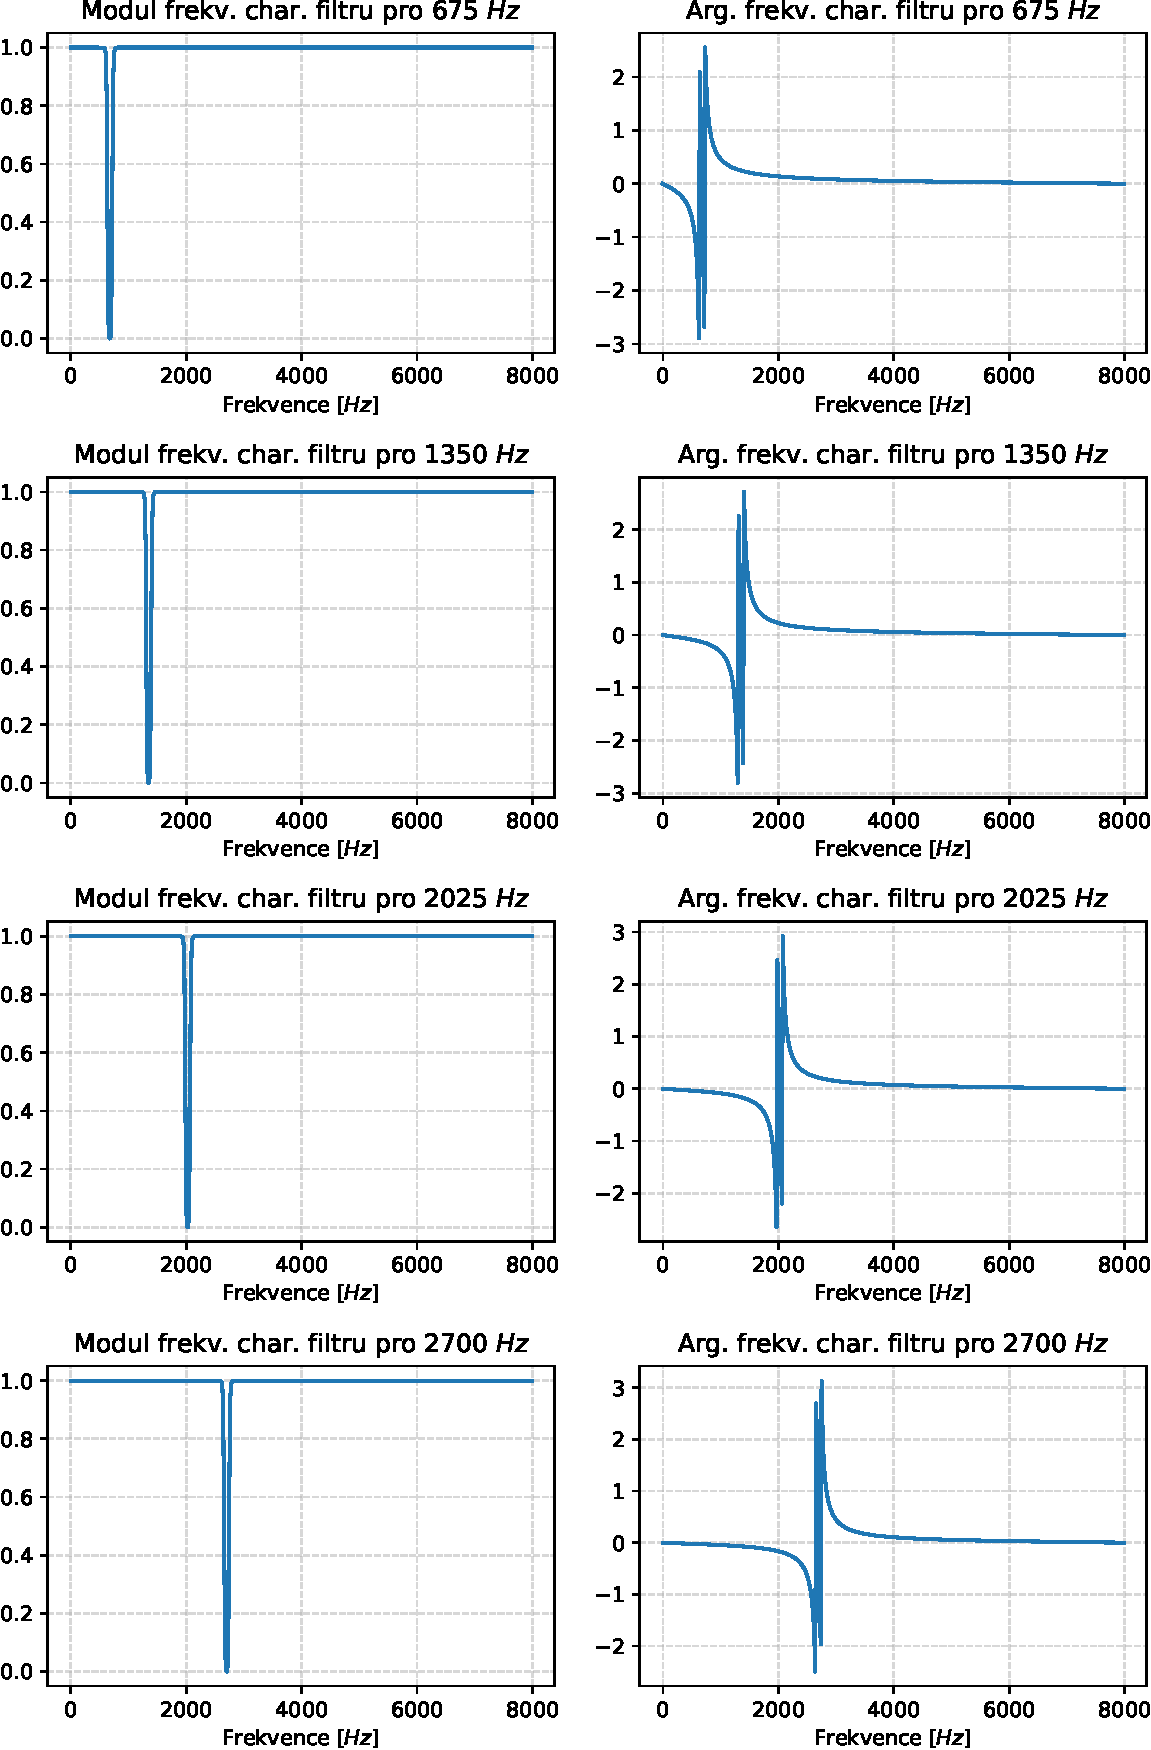
\includegraphics[scale=0.75]{img/09-freq-character.pdf}
    \caption{Frekvenční charakteristiky navržených filtrů}
    \label{fig:filters-freq-character}
\end{figure}



\subsection{Filtrace}
\label{sec:filtration}
Nyní je vypracování projektu téměř u~konce. Zbývá již \uv{pouze} aplikovat navržené filtry na zadaný signál a~ověřit, zda výsledek dopadl podle očekávání. Zhodnocení se věnuji až v~závěru protokolu, tedy v~sekci \ref{sec:end}. Dále budu tedy popisovat jen samotnou aplikaci filtrů a generování konečných výstupů.

Jelikož jsem šel cestou více filtrů typu pásmová zádrž, je o~něco komplikovanější proces samotné filtrace. Tu vykonávám na více částí, kdy se v~každé z~nich aplikuje jeden z~filtrů. Dalo by se to řešit ještě spojením filtrů do~jednoho a poté filtrováním signálu pouze tímto komplexním filtrem, ale to mi přijde jako zbytečně komplikovaný způsob, ve kterém nevidím mnoho pozitiv, jen o~dost práce navíc. Proces filtrování využívá funkci \texttt{lfilter()} z~knihovny SciPy \cite{scipy-reference} a je popsám zdrojovým kódem \ref{code:signal-filtration}. V~dokumentaci se sice píše, že je lepší využít jiné funkce (jako např. \texttt{sosfilt()}), které mají méně numerických problémů, ale i tak jsem se rozhodl použít tuto funkci, protože je využita v~materiálech \cite{zmolikova-demo} a domnívám se, že funguje pro mé účely dostatečně správně.

\begin{lstlisting}[language=Python, caption=Výsledná filtrace zadaného signálu, label={code:signal-filtration}]
filtered_signal = signal

for (b, a) in filters:
    filtered_signal = lfilter(b, a, filtered_signal)
\end{lstlisting}

Dále je třeba vyfiltrovaný signál uložit. Toho se docílí obdobně jako v~případě generovaného signálu s~rušivými kosinusovkami (viz zdrojový kód \ref{code:cos-gen}). Nyní je hotovo. Výslednou zvukovou nahrávku je možné poslechnout a vyzkoušet tak, jak byly filtry úspěšné. Kromě poslechu je však možné ještě vygenerovat graf nového signálu (viz obrázek \ref{fig:filtered-signal-graph}) nebo vygenerovat logaritmický výkonový spektrogram (viz obrázek \ref{fig:filtered-signal-spectrogram}), v~němž je názorně vidět, jak se signál změnil a zda správně vymizely rušivé frekvence.

\begin{figure}[ht]
    \centering
    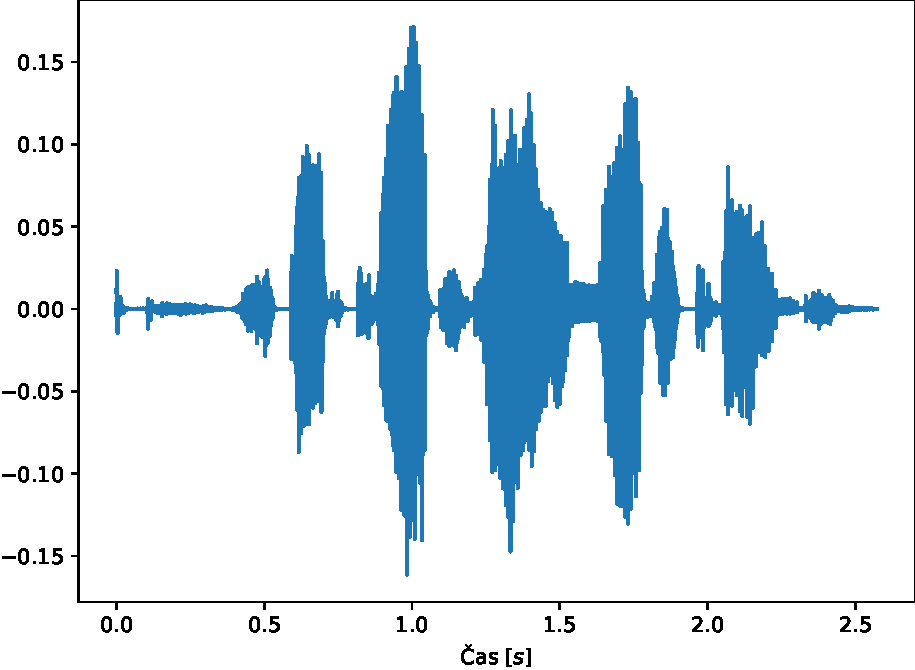
\includegraphics{img/10-filtered-signal.pdf}
    \caption{Graf vyfiltrovaného signálu}
    \label{fig:filtered-signal-graph}
\end{figure}

\begin{figure}[ht]
    \centering
    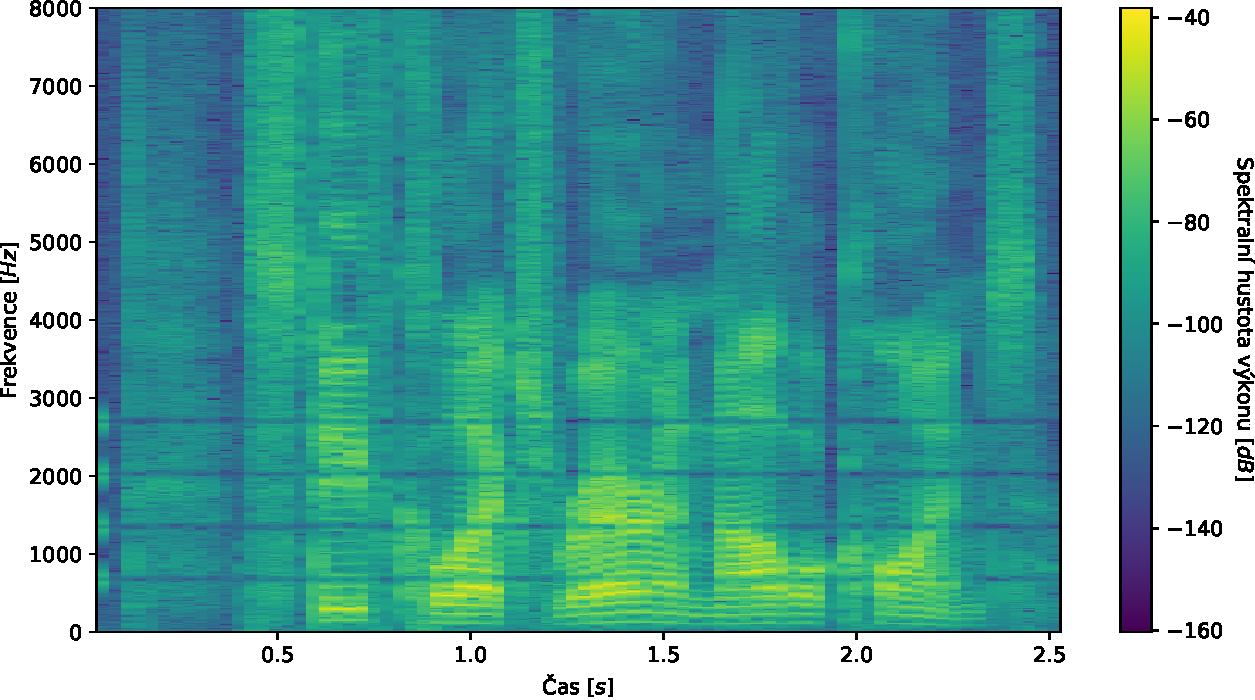
\includegraphics[width=\textwidth]{img/10-final-spectrogram.pdf}
    \caption{Logaritmický výkonový spektrogram výsledného signálu}
    \label{fig:filtered-signal-spectrogram}
\end{figure}

\section{Závěr}
\label{sec:end}

Podle výsledného zvukového signálu a~jeho spektrogramu uvedených v~sekci \ref{sec:filtration} soudím, že se mi filtrace poměrně podařila. Ovšem je zde samozřejmě stále velký prostor pro zlepšení. Frekvence rušivých kosinusovek byly odečteny ručně ze spektrogramu, což není příliš přesné. Filtry nejsou příliš vypilované a~jejich konfigurace je vytvořena pomocí postupu uvedeného v~zadání bez dalšího zkoumání lepších technik. Výsledný zvuk je tedy filtrací postižen drobným poklesem kvality, což může být při pečlivém poslechu znatelné.

Jsem rád, že jsem si mohl vyzkoušet teoretické poznatky z~přednášek na praktickém příkladě a~uvědomit si tak, k~čemu se dá probíraná látka využít v~praxi.

\newpage

\section*{Zdroje}
    \bibliographystyle{czechiso}
    \bibliography{references}

\end{document}
